%%%%%%%%%%%%%%%%%%%%%%%%%%%%%%%%%%%%%%%%%
% baposter Landscape Poster
% LaTeX Template
% Version 1.0 (11/06/13)
%
% baposter Class Created by:
% Brian Amberg (baposter@brian-amberg.de)
%
% This template has been downloaded from:
% http://www.LaTeXTemplates.com
%
% License:
% CC BY-NC-SA 3.0 (http://creativecommons.org/licenses/by-nc-sa/3.0/)
%
%%%%%%%%%%%%%%%%%%%%%%%%%%%%%%%%%%%%%%%%%

%----------------------------------------------------------------------------------------
%	PACKAGES AND OTHER DOCUMENT CONFIGURATIONS
%----------------------------------------------------------------------------------------

\documentclass[landscape,a0paper,fontscale=0.3]{baposter} % Adjust the font scale/size here

\usepackage{graphicx} % Required for including images
\graphicspath{{/home/alli/projects/talks/figures/}} % Directory in which figures are stored

\usepackage{amsmath} % For typesetting math
\usepackage{amssymb} % Adds new symbols to be used in math mode
\usepackage{booktabs} % Top and bottom rules for tables
\usepackage{enumitem} % Used to reduce itemize/enumerate spacing
\usepackage{palatino} % Use the Palatino font
\usepackage[font=small,labelfont=bf]{caption} % Required for specifying captions to tables and figures

\usepackage{multicol} % Required for multiple columns
\usepackage{subcaption}
\usepackage[firstinits=true,backend=bibtex,doi=false,isbn=false,url=false]{biblatex}
\AtEveryBibitem{%
  \clearfield{pages}%
}
\renewcommand{\bibfont}{\normalfont\scriptsize}
\addbibresource{/home/alli/common/refs.bib}

\defbibenvironment{bibliography}
  {\noindent}
  {\unspace}
  {\printtext[labelnumberwidth]{%
    \printfield{prefixnumber}%
    \printfield{labelnumber}}
    \addspace}
\renewbibmacro*{finentry}{\finentry\addspace}

\usepackage{setspace}
\setlength{\columnsep}{1.5em} % Slightly increase the space between columns
\setlength{\columnseprule}{0mm} % No horizontal rule between columns


\usepackage{tikz} % Required for flow chart
\usetikzlibrary{shapes,arrows} % Tikz libraries required for the flow chart in the template

\newcommand{\compresslist}{ % Define a command to reduce spacing within itemize/enumerate environments, this is used right after \begin{itemize} or \begin{enumerate}
\setlength{\itemsep}{1pt}
\setlength{\parskip}{0pt}
\setlength{\parsep}{0pt}
}

\definecolor{lightblue}{rgb}{0.145,0.6666,1} % Defines the color used for content box headers
\definecolor{darkpurple}{rgb}{0.28,0.24,0.55}

\newcommand{\Mod}[1]{\ (\mathrm{mod}\ #1)}



\begin{document}

\begin{poster}
{
headerborder=open, % Adds a border around the header of content boxes
colspacing=1em, % Column spacing
columns=3,
textfont=\Large,
bgColorOne=white, % Background color for the gradient on the left side of the poster
bgColorTwo=white, % Background color for the gradient on the right side of the poster
borderColor=darkgray, % Border color
headerColorOne=darkgray, % Background color for the header in the content boxes (left side)
headerColorTwo=darkpurple, % Background color for the header in the content boxes (right side)
headerFontColor=white, % Text color for the header text in the content boxes
boxColorOne=white, % Background color of the content boxes
%textborder=roundedleft, % Format of the border around content boxes, can be: none, bars, coils, triangles, rectangle, rounded, roundedsmall, roundedright or faded
textborder=rounded, % Format of the border around content boxes, can be: none, bars, coils, triangles, rectangle, rounded, roundedsmall, roundedright or faded
eyecatcher=true, % Set to false for ignoring the left logo in the title and move the title left
headerheight=0.1\textheight, % Height of the header
%headershape=roundedright, % Specify the rounded corner in the content box headers, can be: rectangle, small-rounded, roundedright, roundedleft or rounded
headershape=rounded, % Specify the rounded corner in the content box headers, can be: rectangle, small-rounded, roundedright, roundedleft or rounded
headerfont=\Large\bf\textsc, % Large, bold and sans serif font in the headers of content boxes
%textfont={\setlength{\parindent}{1.5em}}, % Uncomment for paragraph indentation
linewidth=2pt % Width of the border lines around content boxes
}
%----------------------------------------------------------------------------------------
%	TITLE SECTION 
%----------------------------------------------------------------------------------------
%
{\includegraphics[height=6em]{illinois_logo.jpg}} % First university/lab logo on the left
{{Controllable~~Billiards:~~Characterizing~~the~~Paths~~of~~Simple~~Mobile~~Robots}\vspace{-0.0em}} % Poster title
{Alexandra Q. Nilles, Israel Becerra, Steven M. LaValle  \hspace{15pt}\\ Department of Computer Science, University of Illinois, Urbana-Champaign} % Author names and institution
{
\includegraphics[height=8em]{/home/alli/projects/talks/figures/nsf1.jpg}} % Second university/lab logo on the right

%----------------------------------------------------------------------------------------
%	INTRODUCTION
%----------------------------------------------------------------------------------------

\headerbox{Motivation}{name=intro,column=0,row=0,span=1}{
\raggedright
\begin{itemize}\compresslist
\item What {\bf tasks} can simple robots perform?


\item What are the minimal {\bf resources} (sensing, actuation, computation time and
space, feedback control) needed to complete tasks?

\item By leveraging natural dynamics, make robots more efficient
and robust!
\end{itemize}

\begin{center}
\includegraphics[width=0.8\linewidth]{robot_brain.pdf}
\end{center}


}

%----------------------------------------------------------------------------------------
%	Question
%----------------------------------------------------------------------------------------

\headerbox{Robotic Tasks as Properties of Paths}{name=question,below=intro,column=0,span=1}{
\raggedright
\begin{itemize}\compresslist
\item {\bf Navigation:} From a set of starting states, the robot's path must end at the goal state(s).
\item {\bf Coverage:} The robot's path must meet some coverage criterion (scan
some fraction of environment).
\item {\bf Patrolling:} The path must be repeatable, and may also have
some coverage criterion.
\end{itemize}

}

%----------------------------------------------------------------------------------------
%	APPROACH
%----------------------------------------------------------------------------------------


\headerbox{Approach}{name=approach,column=0,span=1,row=3,below=question}{

\begin{itemize}\compresslist
\item Notice that many robots can travel forward in straight lines, identify when
they've reached a boundary, and turn in place.
\item Construct edge-to-edge mapping functions, compose and find
fixed point.
\item See also: aspecular billiards \cite{pinball}, microorganism billiards
\cite{microorganism2017}, bouncing robots \cite{bounce}
\cite{alam2017minimalist}
\end{itemize}


}
%----------------------------------------------------------------------------------------
%	Problem Formulation
%----------------------------------------------------------------------------------------


\headerbox{Modelling One Transition}{name=map,column=1,row=0,span=1}{

\begin{itemize}\compresslist
\item $x$: distance from the nearest clockwise vertex on edge of length $\ell$.
\item Each $n$-sided polygon
and control angle $\theta$ define system of piecewise linear transitions.
\end{itemize}

\vspace{-1.5em}

\begin{equation*}
x_{t+1} = b_{\theta}(x_t) = c (x_t - \ell)   \hskip3em c = \frac{-\cos(\theta)}{\cos(\theta-\phi)}
\end{equation*}


\begin{center}
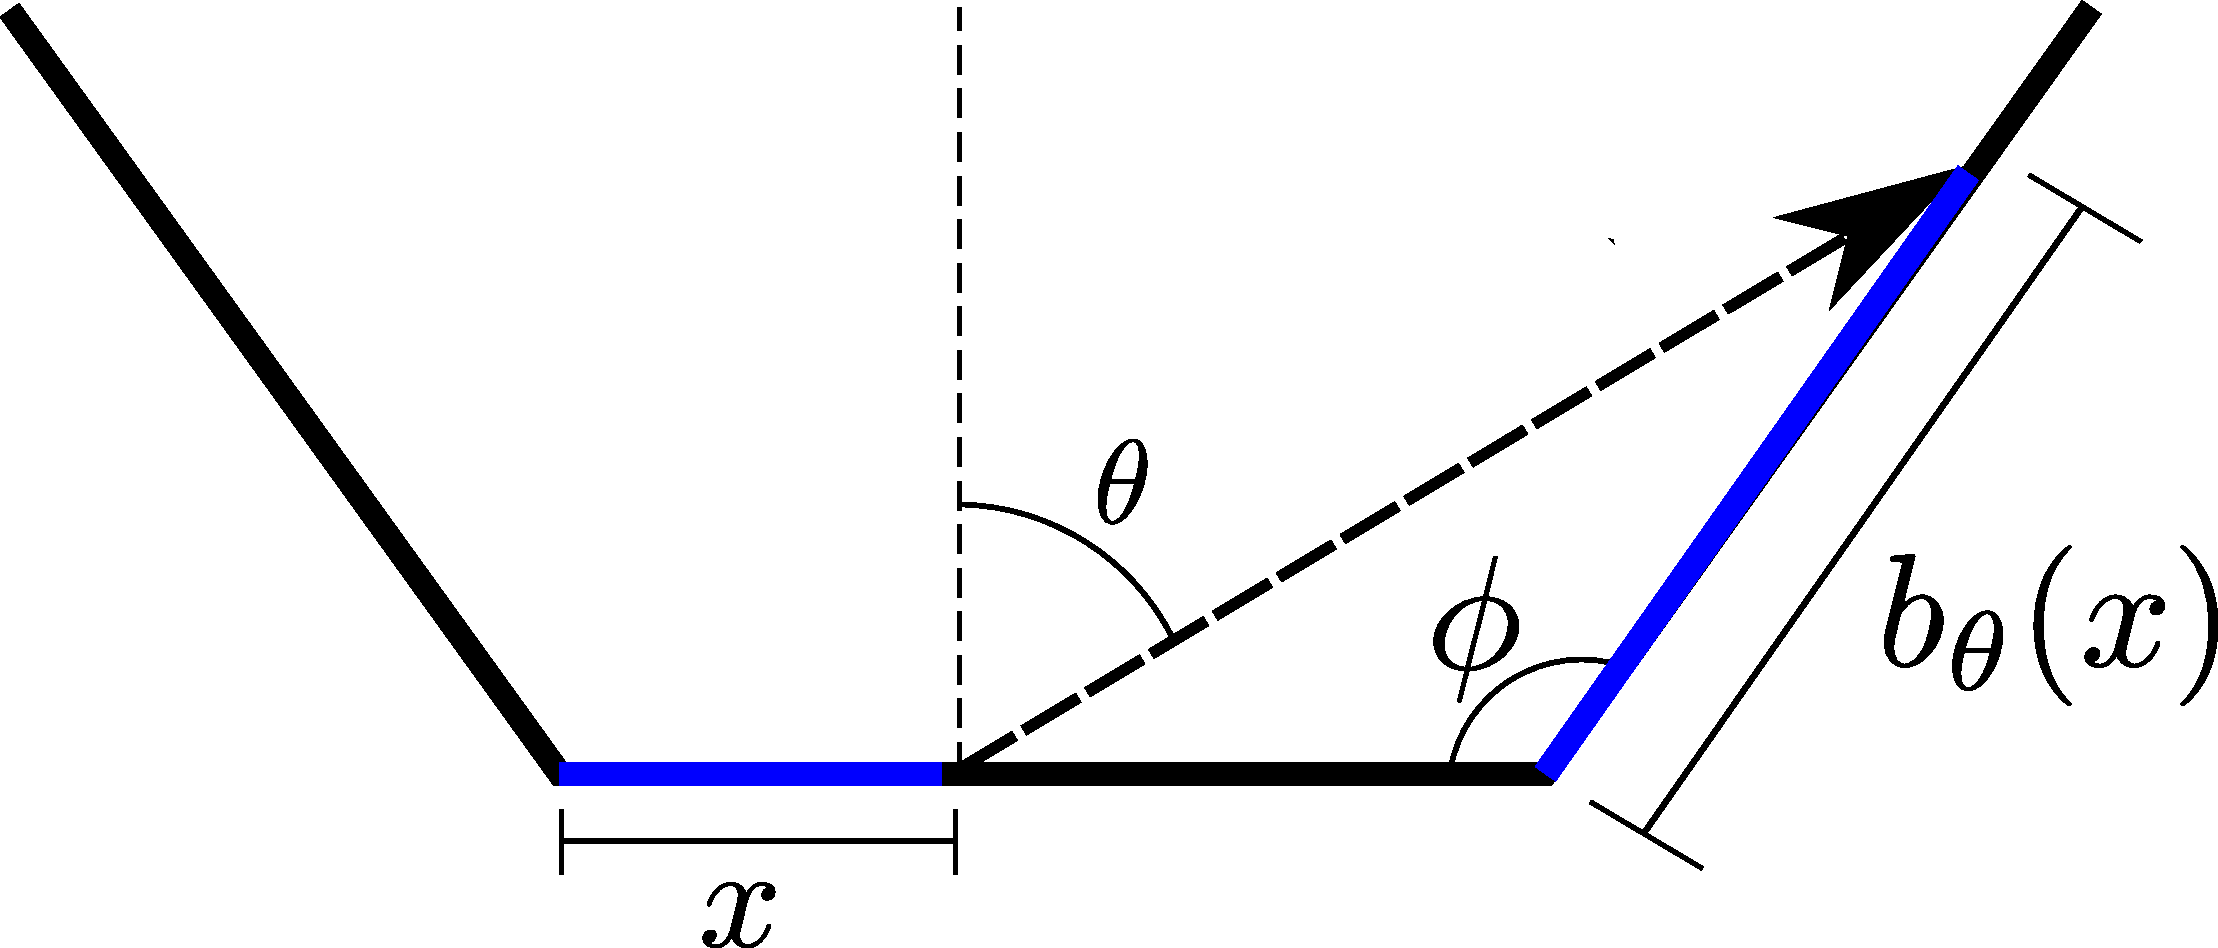
\includegraphics[width=0.7\linewidth]{simple_bounce_def.pdf}
\end{center}

}


%----------------------------------------------------------------------------------------
%	LIMIT CYCLES IN CONVEX POLYGONS
%----------------------------------------------------------------------------------------

\headerbox{Limit Cycles in Convex
Polygons}{name=convex,column=1,bottomaligned=approach,below=map,span=1}{

\begin{itemize}\compresslist
\item Compose edge-to-edge mappings to form $B_{\theta}$, mapping one edge
back to itself.

\item In every convex $n$-sided polygon, there exists a range for $\theta$ such that
$B_{\theta}$ has a fixed point (proof: show that $B_{\theta}$ is a contraction map).
\end{itemize}

\vspace{-0.5em}

\begin{equation*}
x_{FP} = \left(\sum\limits_{i=0}^{n-1} \ell_i \prod\limits_{j=0}^{i-1}
c_j\right)\bigg/ \left(1-\prod\limits_{k=0}^{n-1} c_k\right)
\end{equation*}

\vspace{-1em}

\begin{center}
\includegraphics[width=0.7\linewidth]{convex_fp.pdf}
\end{center}
}

%----------------------------------------------------------------------------------------
%	NONCONVEXITY
%----------------------------------------------------------------------------------------

\headerbox{Ongoing Work: Nonconvexity}{name=nonconvex,column=2,row=0,span=1}{ 


\begin{center}
\includegraphics[width=0.7\linewidth]{nonconvex1.png}
\end{center}

\vspace{-2em}
\raggedright
\begin{itemize}\compresslist
\item Can find "embedded" convex shapes by extending edges: number of potential limit
cycles is exponential in number of sides.
\item How many other limit cycles exist?
\end{itemize}

}

%----------------------------------------------------------------------------------------
%	RESULTS 2
%----------------------------------------------------------------------------------------
\headerbox{Ongoing Work: Coverage
Properties}{name=chaos,column=2,span=1,below=nonconvex}{ 

\begin{multicols}{2}

\begin{center}
\includegraphics[width=0.7\linewidth]{pent_chaos.pdf}
\end{center}

\raggedright
\begin{itemize}\compresslist
\item Are trajectories ergodic?
\item Density of contact with boundary over time?
\end{itemize}

\end{multicols}

}


%----------------------------------------------------------------------------------------
%	FORMAL METHODS
%----------------------------------------------------------------------------------------

\headerbox{Ongoing Work: Verification Tools}{name=fm,column=2,span=1,below=chaos}{

\begin{itemize}\compresslist
\item Formal verification tools can augment analysis of hybrid dynamical
systems.
\item Can express stability as a reachability query: does trajectory ever leave
initial set?
\item Use refinement techniques to find minimal approximation to invariant set?
\end{itemize}

}




%----------------------------------------------------------------------------------------
%	CONCLUSIONS
%----------------------------------------------------------------------------------------



%----------------------------------------------------------------------------------------
%----------------------------------------------------------------------------------------
%	ACKNOWLEDGMENTS
%----------------------------------------------------------------------------------------

\headerbox{Acknowledgments}{name=acknowledgments,column=2,span=1,bottomaligned=convex,
below=fm}{
\footnotesize{
\textbf{Undergraduates}: Michael~Zeng, Yingying~(Samara)~Ren \\
\textbf{Funding}: NSF grants 1035345 and 1328018, and CONACyT
post-doctoral fellowship 277028 \\
%\vspace{-3.5em}
}
\printbibliography[heading=none]


}
%----------------------------------------------------------------------------------------
%	REFERENCES
%----------------------------------------------------------------------------------------

%\headerbox{References}{name=references,column=1,above=bottom}{
%
%\tiny{
%
%
%1. Woese, C., et al. PNAS, 4576–4579 (1990).\\
%2. Zomer, A., et al. PLoS ONE 7, e43012 (2012).\\
%3. Solaimanpour, S., et al. PLOS ONE 10, e0126070 (2015).\\
%4. Makarova, K., , et al. Life 5, 818–840 (2015).
%
%
%}}
%
%----------------------------------------------------------------------------------------
%	FUTURE RESEARCH
%----------------------------------------------------------------------------------------
%
%\headerbox{Future Research}{name=futureresearch,column=1,span=2,aligned=references,above=bottom}{ % This block is as tall as the references block
%
%\begin{multicols}{2}
%Integer sed lectus vel mauris euismod suscipit. Praesent a est a est ultricies pellentesque. Donec tincidunt, nunc in feugiat varius, lectus lectus auctor lorem, egestas molestie risus erat ut nibh.
%
%Maecenas viverra ligula a risus blandit vel tincidunt est adipiscing. Suspendisse mollis iaculis sem, in \emph{imperdiet} orci porta vitae. Quisque id dui sed ante sollicitudin sagittis.
%\end{multicols}
%}
%




\end{poster}

\end{document}
